% ============================================================================
% Reproducible Design-Space Study of Lightweight Lattice-Based Authentication
% and Signatures for Blockchain Transactions
% Technical report (working draft, 2026)
% ============================================================================
\documentclass[11pt]{article}
\usepackage[a4paper,margin=1in]{geometry}
\usepackage[T1]{fontenc}
\usepackage{lmodern}
\usepackage{amsmath,amssymb}
\usepackage{booktabs}
\usepackage{graphicx}
\usepackage{hyperref}
\usepackage[expansion=false]{microtype}
\usepackage{xcolor}
\graphicspath{{../docs/figures_en/}}

\newcommand{\Zq}{\mathbb{Z}_q}
\newcommand{\norminf}[1]{\left\lVert #1 \right\rVert_\infty}

\title{Reproducible Design-Space Study of Lightweight Lattice-Based\\ Authentication and Signatures for Blockchain Transactions}
\author{Zhiqian Lin\\ \small Dalian University of Technology}
\date{\today}

\begin{document}

\maketitle

\begin{abstract}
Quantum computers threaten the classical public-key primitives (RSA, ECDSA) used
by most blockchains today; NIST has therefore standardized lattice-based signatures---ML-DSA (FIPS~204) and
FN-DSA (a FALCON-based scheme being finalized as FIPS~206)---and mandated a transition of the
underlying cryptosystems.  This report describes a \emph{reproducible,
teaching-level} study of the design space of lightweight lattice-based
authentication and signatures for blockchain-style transactions.  We study two
constructions: (i)~Track~A, a symmetric LWE authentication tag whose matrix is
derived per transaction from SHA-256 (``one transaction, one matrix''), and
(ii)~Track~B, a ringless public-key lattice signature in the Lyubashevsky
Fiat--Shamir-with-Aborts style.  Our contribution is methodological rather than
a claim of a new provably secure scheme: we (a)~propose a parameter
instantiation workflow that combines a root-Hermite/core-SVP estimator with
scaled-down LLL embedding attacks and validate the two layers against each
other; (b)~study a message-derived matrix variant that removes the need to
transmit a matrix seed; and (c)~release an open, fully reproducible benchmark
(E1--E4) that follows recent methodological critiques of ML-DSA evaluation by
reporting full latency distributions and rejection-sampling worst cases instead
of means only.  All code, data, seeds, and figures are public.  We do
\emph{not} claim formal security proofs; formal analysis and
module/ring-structured instantiations are left to future work.
\end{abstract}

\section{Introduction}\label{sec:intro}

A growing portion of public ledgers relies on RSA and ECDSA for transaction
authentication.  Shor's algorithm shows that both are broken in polynomial time
on a scalable quantum computer, and NIST has standardized the lattice-based
replacements---ML-DSA (FIPS~204)~\cite{fips204} and FN-DSA, the FALCON-based
  scheme being finalized as FIPS~206~\cite{falcon2020}---
with an explicit recommendation to phase out classical ECC in the near
term~\cite{fips204}.  Recent surveys of post-quantum migration for blockchains
systematically report that lattice signatures inflate transaction and block
sizes (order 10--30$\times$ versus ECDSA) and shift the verification cost
profile~\cite{survey-pq-blockchain-2025,pq-transition-2026}.  In this setting,
the concrete engineering question is not only ``which standard scheme'' but
``how do size, latency, and the sampling behavior of signature algorithms trade
off at a given security level.''  Answering that question carefully requires a
benchmarking methodology that is currently an active research topic in its own
right~\cite{mldsa-bench-2026}.

This work studies two lightweight constructions with the semantics of the
blockchain use case kept explicit:

\begin{itemize}
\item \textbf{Track A --- symmetric LWE authentication tag (MAC).} The issuer
  derives an $n\times n$ matrix $A$ deterministically from the transaction
  payload, computes a tag $b = A s + e \pmod q$ with a short ternary secret $s$,
  and the key-holding verifier checks $\norminf{b - A s} \le V$.  Because
  verification requires the secret $s$, Track A has \emph{MAC semantics}; it
  targets the ``broadcast to a designated offline verifier'' scenario and is
  not directly comparable with public-key signatures.
\item \textbf{Track B --- publicly verifiable lattice signature.} We implement
  a ringless signature in the Lyubashevsky
  Fiat--Shamir-with-Aborts style~\cite{lyubashevsky2009fsa,lyubashevsky2012lswt}:
  the public key is $(A, T = A S)$, the signer masks with a uniform vector and
  rejects until the released vector is short, and anyone can verify without a
  shared secret.
\end{itemize}

Our contributions are:

\begin{enumerate}
\item \textbf{I1 --- parameter methodology with cross-validation.} A
  teaching-level security estimator based on the root-Hermite factor and
  core-SVP costs is used to instantiate parameters at a target security level.
  Because full-size lattice attacks are computationally out of reach on a
  laptop, we additionally run \emph{scaled-down} LLL embedding attacks at
  $q=257$ and verify that the empirically observed key-recovery rate moves in
  the direction predicted by the estimator as dimension, noise, and sample
  count vary.  The two layers of evidence (estimate + phase-transition
  experiment) are meant to be used together; neither is a certificate.  A
  reference lattice-estimator cross-check (Section~\ref{sec:crosscheck})
  quantifies how far the teaching estimate can overshoot in the saturated
  regime and supplies corrected size guidance.
\item \textbf{I2 --- transaction-derived matrix.}  Instead of storing or
  transmitting a matrix seed in the public material, the matrix $A$ is
  expanded from $\mathrm{SHA\text{-}256}(tx)$ with domain separation.  This
  eliminates the seed from the transmitted credential/signature and prevents
  cross-transaction reuse of the same instance.  We explicitly flag the
  security caveat: a message-dependent $A$ lets an adversary choose matrices
  adversarially, which requires an additional reduction argument that is out of
  scope here.
\item \textbf{I3 --- open reproducible benchmark.}  We publish the evaluation
  protocol, seeds, machine metadata, per-sample timing data, rejection-sampling
  histograms, block-inflation estimates, and a one-command reproduction
  pipeline, aligned with the evaluation practices recommended by the recent
  ML-DSA benchmarking critique~\cite{mldsa-bench-2026}.
\end{enumerate}

Scope and honesty statement. This report is a \emph{design-space and
reproducibility study}, not an announcement of a new cryptosystem.  All
security figures are teaching-level estimates of relative hardness trends.  We
deliberately do not report the ``defense-rate'' comparisons of our earlier
prototype (a strawman ``LWE 100\% vs.\ RSA 0\%'' framing), because those two
attacks were not semantically comparable; the discarded material is kept in the
repository only for provenance.

\section{Preliminaries and Related Work}\label{sec:bg}

\subsection{LWE and SIS}
For a prime $q$, the \emph{Learning With Errors} (LWE) problem asks to recover a
secret $s\in\Zq^n$ given $m$ samples $(a_i, b_i = \langle a_i, s\rangle + e_i
\pmod q)$ where $e_i$ is drawn from a (discrete) Gaussian of width $\sigma$.
The \emph{Short Integer Solution} (SIS) problem asks for a nonzero short vector
$x$ in the kernel lattice of a random $A\in\Zq^{m\times n}$.  Both problems
underlie the NIST lattice standards.  We use a ternary secret in
$\{-1,0,1\}^n$ for Track A and a ternary secret matrix in Track B; the security
estimator accounts for the reduced secret entropy as variance.

\subsection{Fiat--Shamir with Aborts}
Lyubashevsky introduced rejection sampling into the Fiat--Shamir transform so
that the released response $z = y + Sc$ is statistically independent of the
secret $S$~\cite{lyubashevsky2009fsa}, and later removed trapdoors from lattice
signatures entirely~\cite{lyubashevsky2012lswt}.  This is the framework used by
CRYSTALS-Dilithium/ML-DSA.  Recent academic work continues to compress
signatures and reduce sampling cost in this framework: HAETAE uses bimodal
rejection sampling~\cite{haetae2024}, G+G removes rejection sampling via
convolved Gaussians~\cite{gg2023}, Rhyme proposes a 3C sampling that avoids
flooding, rejection sampling, and Gaussian convolution~\cite{rhyme2025}, and a
very recent line achieves the first tight reductions from
\emph{search-LWE} without trapdoors~\cite{tightlwe2026}.  Our Track B is a
deliberately simple, ringless reference implementation in the same
Fiat--Shamir-with-Aborts family; it is a baseline for methodology, not a
competitor to these optimized schemes.

\subsection{Benchmarking methodology}
Riou et al.\ show that ML-DSA signing time is highly variable because of
rejection sampling, and that reporting only means systematically underestimates
worst-case execution time by up to roughly $20\times$~\cite{mldsa-bench-2026}.
They recommend fixed input sets, per-sample timing, and reporting quantiles and
worst cases rather than single-point averages.  We follow that protocol in
E2/E4 and additionally release the raw samples so that empirical CDFs can be
recomputed.

\subsection{Blockchain migration surveys}
Surveys of post-quantum blockchains consistently identify signature size as the
dominant driver of ledger inflation and quantify verification overhead against
the ECDSA baseline~\cite{survey-pq-blockchain-2025,pq-transition-2026}.  We use
their reporting conventions (bytes, block-inflation multiple, verify TPS) in
the blockchain scenario experiment E4.

\section{Constructions and Threat Models}\label{sec:constr}

All arithmetic is over $\Zq$ with a prime $q=12289$ (12-bit modulus used by
many lattice instantiations) unless stated otherwise.  Deterministic expansion
uses SHA-256 with domain separation and a counter-mode PRG; the implementation
is documented in the repository.

\subsection{Track A: symmetric LWE authentication tag}\label{sec:tracka}

Parameters: $n$, $q$, $\sigma$ (Gaussian width), tail $t$, and verification
tolerance $V$.  Setup chooses a uniform ternary secret $s \in \{-1,0,1\}^n$.
For a transaction $tx$:
\begin{enumerate}
\item \textbf{Derive} $A = \text{Expand}(\mathrm{SHA\text{-}256}(\texttt{tag-domain} \| tx)) \in \Zq^{n\times n}$;
\item \textbf{Issue} $b = A s + e \pmod q$, where each $e_i$ is drawn from a
  truncated discrete Gaussian of width $\sigma$ and support $\{-t,\dots,t\}$;
\item \textbf{Verify} (key holder only): recompute $A$ from $tx$ and accept iff
  $\norminf{b - A s} \le V$.
\end{enumerate}
Because the verifier needs $s$, Track A is a \emph{message authentication tag},
not a digital signature.  It is appropriate for ``broadcast to a designated
verifier with an established shared key''; it cannot provide public
verifiability or non-repudiation.  Its adversary goal is existential
forgeability of a fresh tag from observed $(tx_i, b_i)$ transcripts, i.e., a
\emph{search-LWE} instance over the collected samples.

\subsection{Track B: publicly verifiable lattice signature}\label{sec:trackb}

Parameters: $A \in \Zq^{m_a \times n}$ with $m_a=224$ rows and $n=256$
dimensions, secret $S\in \{-1,0,1\}^{n\times m_c}$ with $m_c=256$ (each entry
nonzero with probability $2/3$), challenge length $m_c=256$ and Hamming weight
$h=32$, mask radius $\kappa$, acceptance bound $\kappa - h$, and hash
$H = \mathrm{SHA\text{-}256}$.  The public key is $(A, T = A S \bmod q)$.
Keygen, sign, and verify are:

\begin{enumerate}
\item \textbf{Keygen:} sample $A$ uniformly from a seed, sample the ternary
  secret matrix $S$, and set $T = A S \bmod q$.
\item \textbf{Sign($tx$):} repeat: (1)~sample $y \in [-\kappa,\kappa]^n$
  uniformly and compute $w = A y \bmod q$; (2)~compute the digest
  $c = H(tx \| \text{encode}(w))$ and expand it into a sparse ternary challenge
  vector with Hamming weight $h$; (3)~set $z = y + S c$ and \emph{accept} only
  if $\norminf{z} \le \kappa - h$; otherwise restart.  Output the signature
  $(z, \text{digest})$.
\item \textbf{Verify($tx$, $(z,\text{digest})$):} reject if
  $\norminf{z} > \kappa-h$; recompute $c$ from the digest; accept iff
  $H(tx \| \text{encode}(A z - T c)) = \text{digest}$.
\end{enumerate}

Correctness follows from $A z - T c = A y + A S c - A S c = w \bmod q$.
Conditioned on acceptance, $z = y + S c$ is uniformly distributed over
$[-\kappa+h, \kappa-h]^n$ and is independent of $S$ (statistical
zero-knowledge), because $y$ is uniform and the map $y \mapsto z$ is a
bijection on the acceptance region.  Forging a signature requires finding a
short $S'$ with $A S' = T \pmod q$, an \emph{inhomogeneous} SIS instance.  All
of these statements are standard textbook arguments; we make no claim of new
cryptanalysis.  As discussed below, the ringless instantiation has a large
public key ($\approx 224$~KB), which motivates module/ring structure in a
production design.

\subsection{Semantic boundaries}
\begin{table}[t]
\centering
\caption{Semantics of the two constructions studied in this paper.}
\label{tab:semantics}
\small
\begin{tabular}{@{}lllp{4.7cm}@{}}
\toprule
Scheme & Semantics & Verifier & Attack model \\
\midrule
Track A (tag)   & MAC (symmetric)  & key holder only & forge fresh tag from $(tx_i,b_i)$ transcripts \\
Track B (sig.)  & digital signature & any party & find short $S'$ with $A S'=T$ \\
RSA/ML-DSA/FN-DSA & digital signature & any party & standard baselines \\
\bottomrule
\end{tabular}
\end{table}
Keeping these boundaries explicit avoids the common trap of comparing a
symmetric MAC against public-key signatures on ``who prevents forgery better'';
instead Track A is positioned for symmetric, key-holder-checked settings, and
only Track B is placed on the same comparison plane as RSA-PSS and the NIST
schemes.

\section{Parameter Methodology (I1)}\label{sec:method}

\subsection{Teaching-level security estimator}
For an LWE instance with $n$ dimensions, $m$ samples, modulus $q$, Gaussian
width $\sigma$, and ternary secret variance $2/3$, we model the best known
attack as a Kannan embedding into a lattice of dimension $d = m + n + 1$.  The
required root-Hermite factor is compared against the achievable factor of BKZ-$\beta$,
\[
\delta(\beta) = \left( \frac{\beta}{2\pi e} (\pi\beta)^{1/\beta} \right)^{1/(2(\beta-1))},
\]
and the core-SVP cost is taken as $2^{0.292\beta}$ (classical) or
$2^{0.265\beta}$ (quantum), following the NewHope cost model.  For a target of
$\geq 80$ bits this scan returns $n = m = 144$, $q = 12289$, $\sigma = 2$,
tail $t=6$, $V=8$, with an estimate of $84.4$ bits at full-dimension block size
$\beta = 289$.  As quantified in Section~\ref{sec:crosscheck}, this figure is
the estimator's \emph{dimensional-saturation ceiling}, not a supported security
estimate: the reference lattice-estimator puts the same instance at roughly
$2^{12}$--$2^{41}$ of attack cost.  For Track B we check the SIS regime: with $n=256$ dimensions
and $m_a=224$ rows the target norm lies about $-30.5$~dB below the Gaussian
heuristic bound, i.e., in the region where finding a short solution requires
lattice reduction.

\begin{figure}[t]
  \centering
  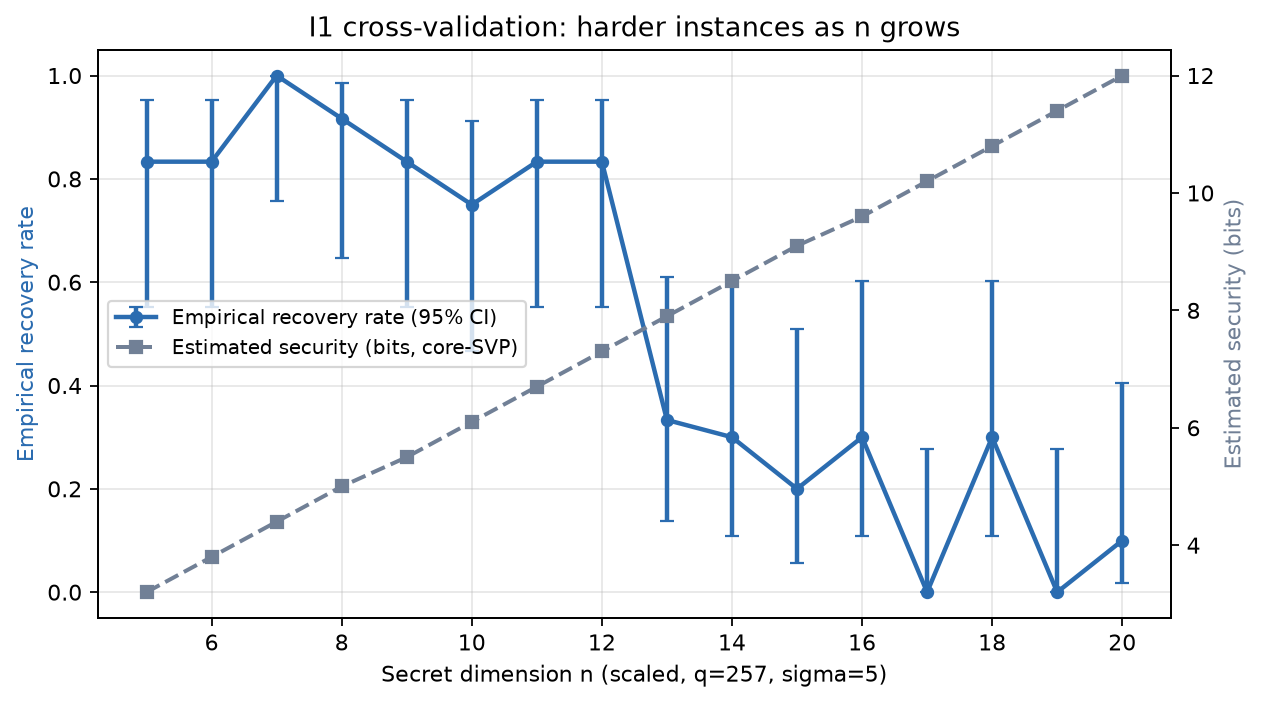
\includegraphics[width=0.8\linewidth]{fig2_nsweep.png}
  \caption{I1 cross-validation (scaled, $q=257$, $\sigma=5$): the empirical
  key-recovery rate of a Kannan-embedding LLL attack (left axis, 95\% Wilson
  CI) decreases as the secret dimension $n$ grows, while the teaching
  estimator's bit-security (right axis) increases.  Each point: 8--12
  independent instances.}
  \label{fig:n}
\end{figure}

\begin{figure}[t]
  \centering
  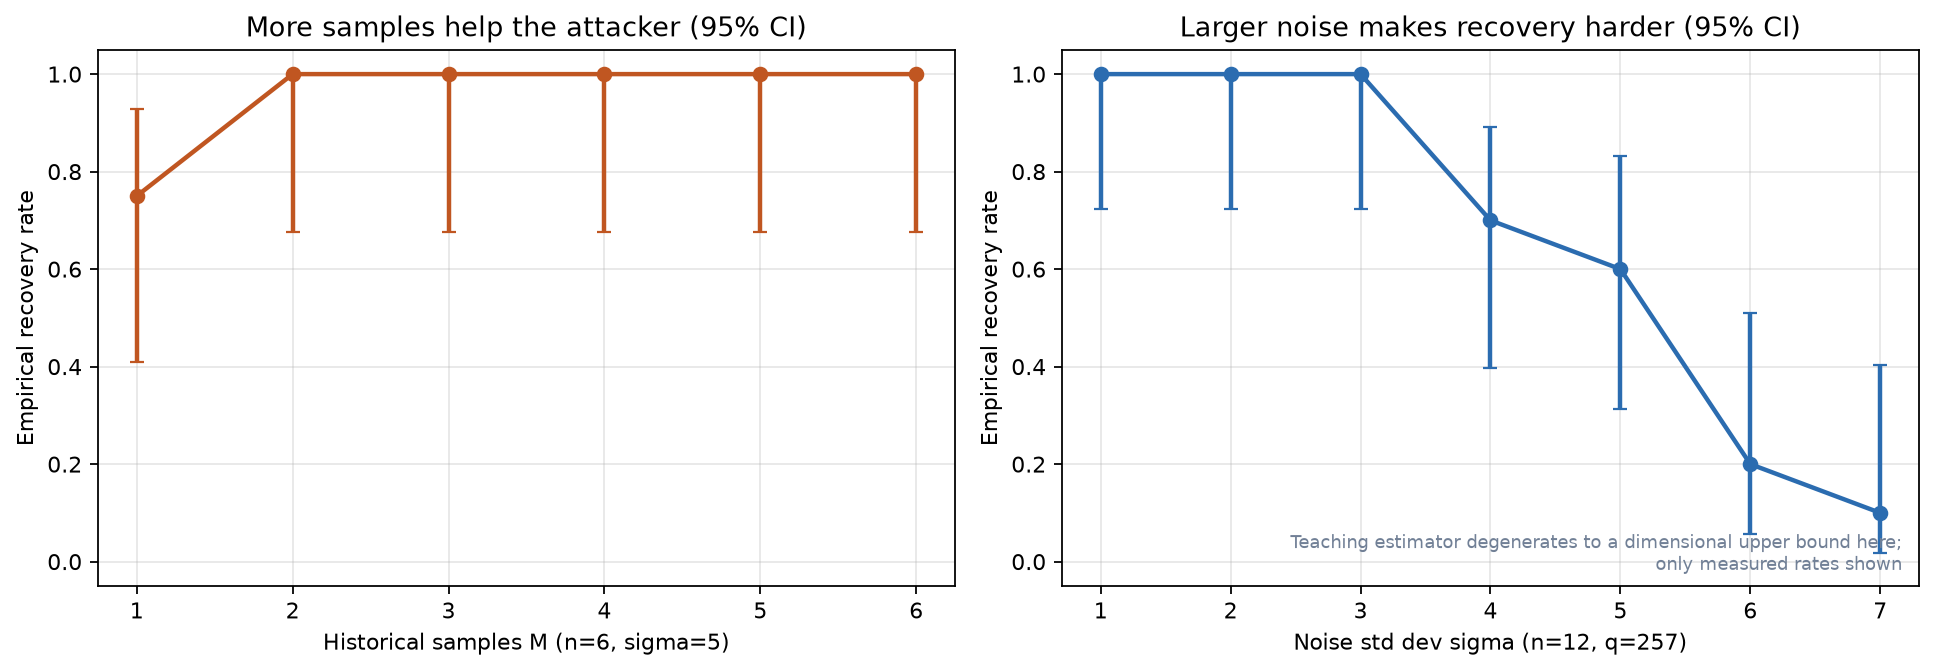
\includegraphics[width=\linewidth]{fig3_msigma.png}
  \caption{Left: recovery rate vs.\ the number of historical LWE samples $M$
  ($n=6$, $\sigma=5$); more samples help the attacker.  Right: recovery rate
  vs.\ noise width $\sigma$ ($n=12$); larger noise makes recovery harder.  In
  this low-dimensional teaching regime the estimator degenerates to a
  dimensional bound, so only measured rates (with 95\% Wilson CI) are shown.}
  \label{fig:m}
\end{figure}

\subsection{Scaled-down cross-validation}
Directly attacking the full-size parameters is out of reach, so we validate
trends on scaled instances with $q=257$ and $\sigma=5$ so that the target/GH
ratio is near 1 and phase transitions are observable in small dimensions.  Our
attack is a self-contained Kannan embedding using a QR-accelerated floating
point LLL (dimensions $\le 41$), followed by Babai nearest-plane decoding; each
parameter point uses 8--12 independent random instances with a 120\,s time
budget per point.  We sweep (a)~secret dimension $n \in \{5,\dots,20\}$,
(b)~the number of historical samples $M \in \{1,\dots,6\}$ at fixed $n=6$, and
(c)~the noise width $\sigma \in \{1,\dots,7\}$ at fixed $n=12$.  Section
\ref{sec:results} reports that the measured success rates move \emph{in the
direction} predicted by the estimator (harder as $n$ grows or $\sigma$ grows;
easier as $M$ grows).  This is a consistency check of the estimation
\emph{trends}, not a security proof for any concrete parameter set.
Section~\ref{sec:crosscheck} reports a reference lattice-estimator
cross-check that quantifies how far the teaching model can overshoot in the
saturated regime and gives corrected size recommendations.

\subsection{Reference cross-check with lattice-estimator}\label{sec:crosscheck}

To obtain an independent reference point, we evaluate the Track~A and Track~B
instances with the community lattice-estimator~\cite{albrecht2018estimator}
(git commit \texttt{53da598}, 2026-08-19).  The tool is normally distributed
as a SageMath package; to keep this artifact dependency-light we executed its
attack code \emph{unmodified} under CPython through a small pure-Python layer
that re-implements the handful of \texttt{sage.all} numerical symbols the
package imports (53-bit reals with an MPFR-scale exponent range, integer and
rational rings, binomial/log/erf, and the normal/\textsuperscript{$\chi^2$}
CDFs).  The layer is validated against the estimator's own doctest reference
values before any new numbers are produced; Table~\ref{tab:xcheck-validation}
shows that every reference row reproduces exactly at the printed precision.
We report four attack families: primal uSVP and BDD under the estimator's
default reduction-cost model, and uSVP plus dual-hybrid under the ADPS16
core-SVP / GSA model used by \texttt{estimate.rough} (the
literature-comparable numbers).  We do not report the default-model full
\texttt{dual} family: that routine internally amplifies success probabilities
below the IEEE-754 range, where only Sage's MPFR semantics apply; its
conservative core-SVP analogue (rough dual-hybrid) is included instead.

\begin{table}[h]
\centering
\small
\setlength{\tabcolsep}{3pt}
\caption{Validation of the numerical layer.  Reference values are the
lattice-estimator doctest outputs; ``this work'' values come from identical
calls in this artifact.  All rows match at the printed precision
($\pm0.1$~bit).}
\label{tab:xcheck-validation}
\begin{tabular}{lcccc}
\toprule
Instance & Call & ref.\ cost ($\log_2$) & ref.\ $\beta$ / $d$ & this work \\
\midrule
Kyber512       & uSVP (default)        & $143.8$ & 406 / 998  & same \\
Kyber512       & BDD (default)         & $140.2$ & 389 / 1005 & same \\
Kyber512       & uSVP (ADPS16/GSA)     & $118.6$ & 406 / 998  & same \\
Dilithium2 MSIS & SIS lattice (rough)  & $123.5$ & 423 / 2303 & same \\
\bottomrule
\end{tabular}
\end{table}

\paragraph{Track A.} Table~\ref{tab:xcheck-tracka} reports the reference
costs for the benchmarked prototype ($n=m=144$) and for $n=m=480$, the
smallest size in our scan at which the conservative ADPS16 uSVP estimate
reaches $\approx 91$ bits.  Under the reference estimator the $n=144$
prototype is worth only $\approx 2^{41}$ (default uSVP/BDD) to $\approx 2^{12}$
(core-SVP uSVP) word operations---far below the $84.4$ bits of the teaching
scan, which saturates at its dimensional ceiling ($\beta=d=289$).  The
teaching estimator is therefore a \emph{loose upper bound} in this regime, not
a security estimate, and the agreement seen in E3 is a validation of
\emph{trends} rather than of absolute cost.  The default-model scan reaches 80
bits at $n\approx 320$, but the conservative core-SVP rows require
$n\approx 440$--$480$; we therefore recommend $n=m=480$, $q=12289$,
$\sigma=2$ as a ${\sim}90$~bit teaching instantiation of Track~A
(Figure~\ref{fig:crosscheck}).  All E1--E4 benchmark data in this report keep
the original $n=144$ prototype and are methodology-level, not
security-level, data.

\begin{table}[h]
\centering
\small
\setlength{\tabcolsep}{3pt}
\caption{Reference lattice-estimator costs for the Track~A LWE-tag family
($q=12289$, $\sigma=2$, independent ternary secret, $m=n$).  Values are
$\log_2$ word operations of the cheapest reported row per family.}
\label{tab:xcheck-tracka}
\begin{tabular}{lcccc}
\toprule
$n$ & uSVP (default) & BDD (default) & uSVP (ADPS16) & dual-hybrid (ADPS16) \\
\midrule
144 (prototype)   & $41.3$ & $41.1$ & $12.0$ & $17.7$ \\
480 (recommended) & $117.9$ & $114.8$ & $91.4$ & $89.4$ \\
\bottomrule
\end{tabular}
\end{table}

\begin{figure}[h]
  \centering
  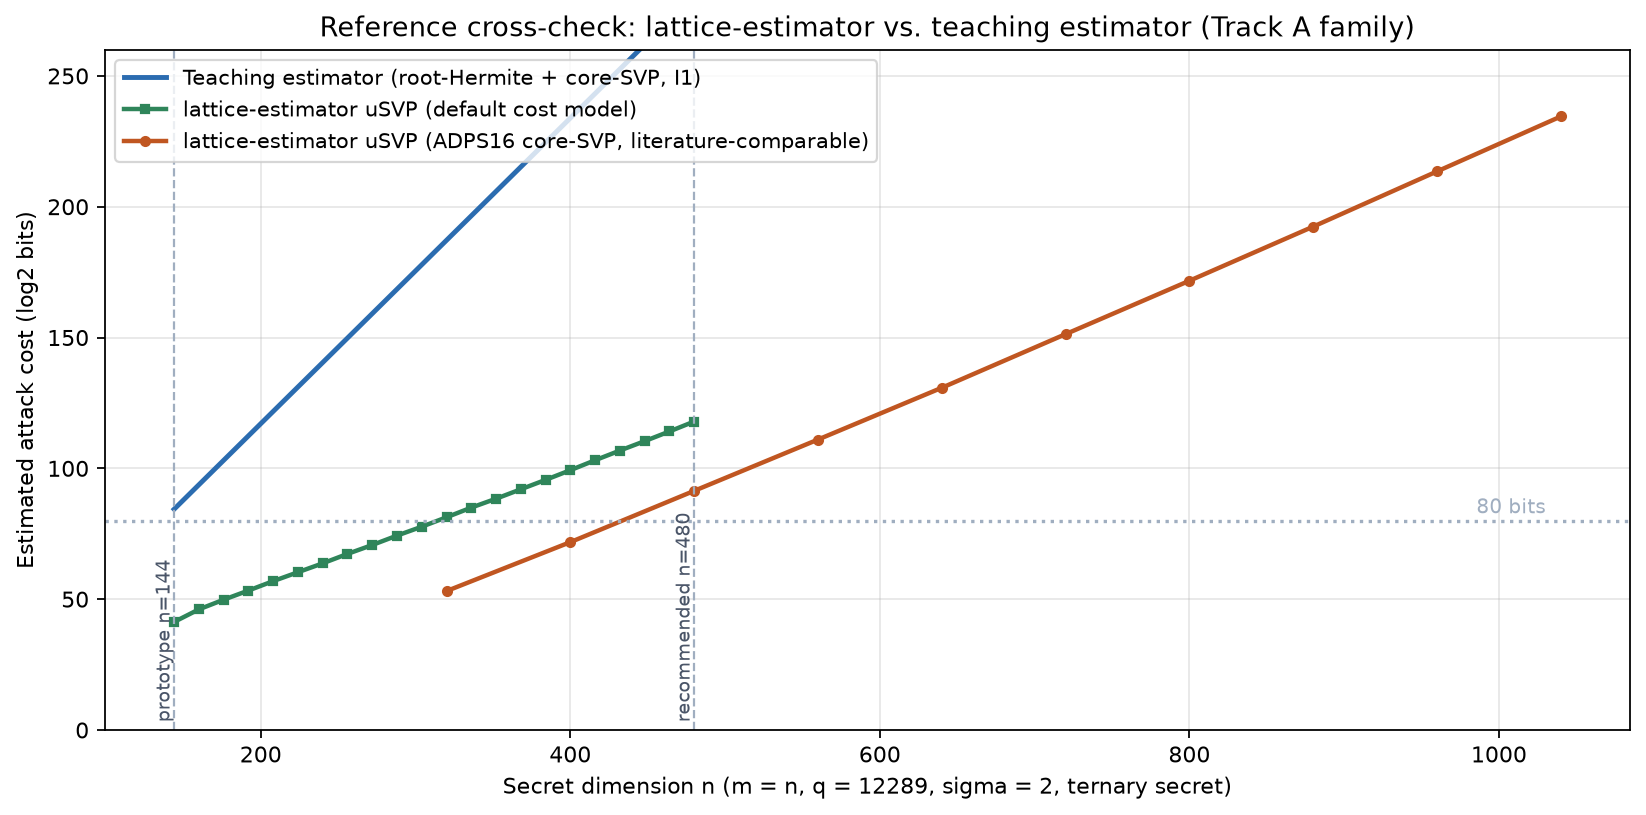
\includegraphics[width=0.92\linewidth]{fig7_reference_bits.png}
  \caption{Reference cross-check on the Track~A family.  The teaching
  root-Hermite/core-SVP estimator (blue) grows linearly with the secret
  dimension because it saturates at block size $\beta=d=2n+1$; the reference
  lattice-estimator uSVP estimates under the default model (green) and under
  the ADPS16 core-SVP model (orange) are far lower at the benchmarked
  $n=144$.  A prototype of $n=480$ clears ${\sim}80$ bits under both reference
  models.}
  \label{fig:crosscheck}
\end{figure}

\paragraph{Track B.} We cross-checked the SIS core used by the methodology,
namely the homogeneous kernel of the $224\times256$ matrix $A$ with the
Euclidean bound $\sqrt{256\cdot 2/3}\approx13.1$ of a planted ternary
column.  The reference lattice attack reports \emph{no} admissible vector
(cost $2^{\infty}$, $\beta=d=224$): for a uniformly random matrix the
Gaussian-heuristic shortest vector of this $q$-ary lattice is
$\lambda_1\approx1.5\times10^4$, so no $13$-bounded kernel vector exists in
the generic model.  This confirms that the relevant hardness of Track~B is the
\emph{planted, inhomogeneous} (preimage) problem, which the reference tool does
not model directly, and it explains why Track~B is reported ``in the SIS
regime'' without a claimed bit count.  Two design constraints follow for future
parameter derivation.  First, the infinity-norm MSIS attack in the reference
tool requires the length bound to stay below $(q-1)/2=6144$; the
two-signature relation of Section~\ref{sec:trackb} can have coordinates up to
$2(\kappa-h)=7848$, so parameter selection must either reduce $\kappa-h$ or
increase $q$ until $2(\kappa-h)<(q-1)/2$.  Second, a bit-level instantiation
of the inhomogeneous instance (e.g.\ via module structure as in ML-DSA) is
left to future work.

\section{Transaction-Derived Matrix (I2)}\label{sec:i2}

Lattice schemes such as ML-DSA expand a short random \emph{seed} into the
matrix $A$ so that the public key carries only the seed.  I2 applies the same
idea at the message level: for Track A (and similarly for Track B challenges),
we derive the matrix from the transaction hash with a domain-separation prefix,
\[
A_{tx} = \text{Expand}(\mathrm{SHA\text{-}256}(\texttt{domain} \| tx)).
\]
This has two engineering consequences.  First, no matrix seed needs to be
transmitted or stored alongside the credential, since every verifier can
recompute $A_{tx}$; the tag/signature remains compact.  Second, because $A$
changes with the transaction, an adversary cannot amortize one instance across
many signed messages; E3(b) confirms empirically that accumulating samples from
the same instance makes key recovery markedly easier (Section
\ref{sec:results}), which is exactly the reuse that per-transaction derivation
prevents.

\emph{Security caveat.} Making $A$ a function of the message gives the
adversary some control over the matrix by choosing messages, so the reduction
must account for adversarially chosen $A$.  A full treatment (e.g., randomizing
the derivation or proving hardness under a suitable variant) is future work.
We therefore present I2 as an engineering feasibility study with a clearly
stated boundary, not as a proven construction.

\section{Experimental Evaluation}\label{sec:eval}

\subsection{Environment and protocol}
All experiments run single-threaded on a Windows 11 desktop (AMD desktop CPU, Family 25 Model 68,
Python 3.12.10, NumPy 2.5.3, matplotlib 3.11.1, OpenSSL 3.5.7), with machine
metadata embedded in the result JSON files.  Timing uses
\verb|time.perf_counter| and includes Python call overhead; the RSA baseline is
measured with OpenSSL's in-process \verb|openssl speed| (industry-standard
implementation), and per-sample distributions are unavailable there, so it is
marked as constant.  All random seeds are fixed (E1: 12345; E1b/E2: 20260908; E3: 20260908) and the
entire pipeline runs with
\verb|python scripts/run_v2_all.py|.

\subsection{E1: correctness and threshold behavior (Track A and Track B)}
For $n=144$, $q=12289$, $\sigma=2$, $V=8$, we test 1500 valid transactions,
1500 bit-flipped tampered transactions, and 300 random blind tags.  All 1500
valid tags are accepted, all 1500 tampered transactions are rejected, and all
300 blind tags are rejected (each rate $= 1.0000$).  Figure~\ref{fig:e1} (left)
shows that verification residuals of valid tags concentrate in
$[5,6]$ (mean $5.45$, max $6$) while tampered transactions produce residuals
far above the threshold.  The right panel sweeps $V\in\{0,\dots,16\}$: the
false-reject rate is $1.0$ for $V\le 3$, $0.959$ at $V=4$, $0.494$ at $V=5$,
and $0$ for $V\ge 6$, while the tamper-pass rate is $0$ across the entire
sweep.  Choosing $V=8$ leaves a comfortable margin below the empirical
residual maximum of 6.

\begin{figure}[t]
  \centering
  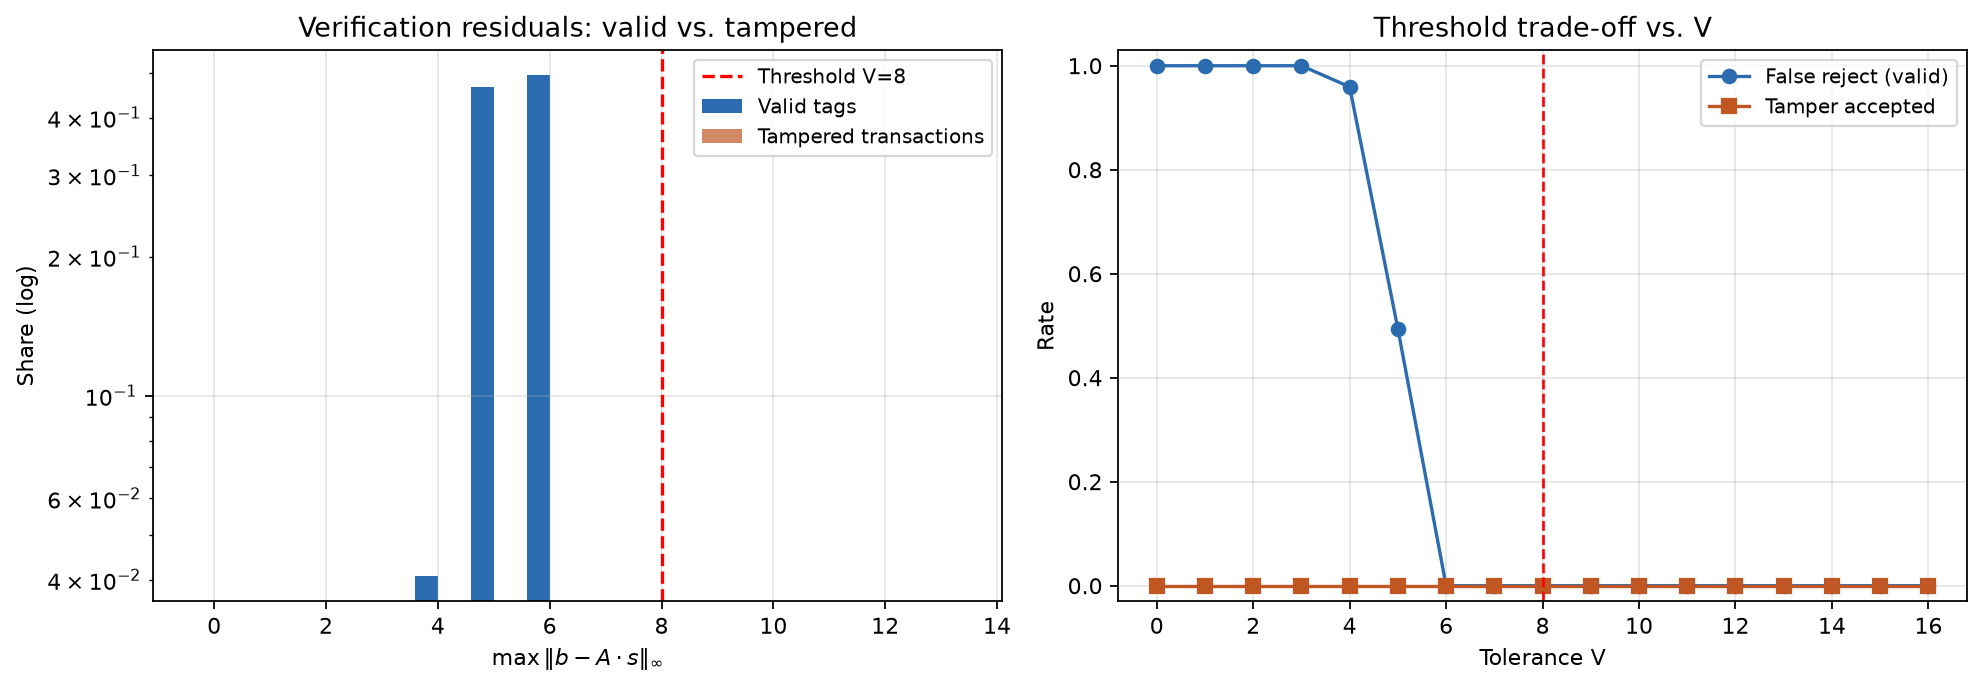
\includegraphics[width=\linewidth]{fig1_correctness.png}
  \caption{E1 (Track A).  Left: normalized histogram (log scale) of
  verification residuals $\norminf{b - A s}$ for valid tags and for tampered
  transactions (V$=8$); residuals of tampered transactions exceed the
  histogram range shown here.  Right: false-reject rate (valid) and
  tamper-pass rate vs.\ tolerance $V$.}
  \label{fig:e1}
\end{figure}

\paragraph{Track B correctness.} At the prototype scale used in E2
($n=256$, $m_a=224$, $h=32$, $\kappa=3956$), we additionally test
Track B in four groups of 1000 trials: (i)~all valid signatures
verify; (ii)~all bit-flipped transactions are rejected; (iii)~all
random forgeries---uniform random $z$ with $\norminf{z}\le\kappa-h$ and
a fresh 32-byte digest---are rejected; and (iv)~all signatures mutated
in a single byte are rejected (each rate $= 1.0000$).  Unit tests in
the repository cover the same round-trip and tamper paths at smaller
scale.  Result JSON: \texttt{data/eval\_v2\_e1b.json}.

\subsection{E3: scaled attacks (I1 cross-validation)}\label{sec:results-e3}
Figure~\ref{fig:n} sweeps the secret dimension $n$ at $q=257$, $\sigma=5$: the
measured recovery rate falls from $0.83$ at $n=5$ to $0.10$ at $n=20$ (per-point
95\% Wilson intervals; small-sample noise between adjacent points is expected),
while the estimator rises from $3.2$ to $12.0$ estimated bits.  Figure
\ref{fig:m} (left) fixes $n=6$ and varies the number of samples: recovery rises
from $0.75$ ($M=1$) to $1.0$ ($M\ge 2$), confirming that accumulating samples
from the \emph{same} instance favors the attacker.  Figure~\ref{fig:m} (right)
fixes $n=12$ and varies $\sigma$: recovery drops from $1.0$ ($\sigma\le3$) to
$0.1$ ($\sigma=7$).  The qualitative agreement between the empirical phase
transitions and the estimator is the central evidence for I1.

\subsection{E2: prototype size and latency comparison}
Table~\ref{tab:perf} summarizes sizes and latencies.  All rows use the
teaching-level instantiations of Section~\ref{sec:method} (Track A:
teaching estimate $84.4$ bits, but the reference cross-check of
Section~\ref{sec:crosscheck} puts the $n=144$ prototype at roughly
$2^{12}$--$2^{41}$; Track B: reported in the SIS regime without a claimed bit
count; RSA-3072: $\approx112$ bits), so the rows are not at a matched
security level.  Track B signing has
median $1.36$~ms but a heavy tail ($p_{90}=4.49$~ms, $p_{99}=9.66$~ms,
max $24.1$~ms) driven by rejection sampling; the number of retries per
signature has median 6 and reaches 61 in the worst case.  Figure~\ref{fig:perf}
(left) shows the empirical CDFs of signing time, where the Track B long tail is
clearly visible against the near-constant Track A and RSA values.  Verification
is fast for all schemes ($\le 0.16$~ms median here).  Track A ``signing''
(issuing the tag) has median $2.34$~ms and p99 $4.99$~ms; its low p99/max
spread reflects the absence of rejection sampling.

\begin{table}[t]
\centering
\small
\setlength{\tabcolsep}{4pt}
\caption{Size and timing comparison.  Rows for Track A/B and RSA-3072-PSS are
measured on this machine; the NIST rows use official sizes---ML-DSA-44 (FIPS
204) and FN-DSA-512 (FALCON v1.2, the scheme planned as FIPS 206)---and are not
measured here.  Security levels are teaching-level and not matched across rows.  Signing medians with p99 in parentheses; verify
median.  Sig. = signature or credential.}
\label{tab:perf}
\begin{tabular}{lccccl}
\toprule
Scheme & pk (B) & sk (B) & sig/cred (B) & sign med (ms) & verify med (ms) \\
\midrule
Track A tag (symmetric) & --- & 144 & 288 & 2.34 (p99 4.99) & 0.098 \\
Track B signature (ringless) & 229\,376 & 65\,536 & 544 & 1.36 (p99 9.66) & 0.160 \\
RSA-3072-PSS (OpenSSL 3.5.7) & 384 & 384 & 384 & 7.39 & 0.135 \\
ML-DSA-44 (official) & 1312 & 2560 & 2420 & ref. & ref. \\
FN-DSA-512 (FALCON) & 897 & 1281 & 666 & ref. & ref. \\
ECDSA P-256 (official) & 65 & 32 & 64 & ref. & ref. \\
\bottomrule
\end{tabular}
\end{table}

\begin{figure}[t]
  \centering
  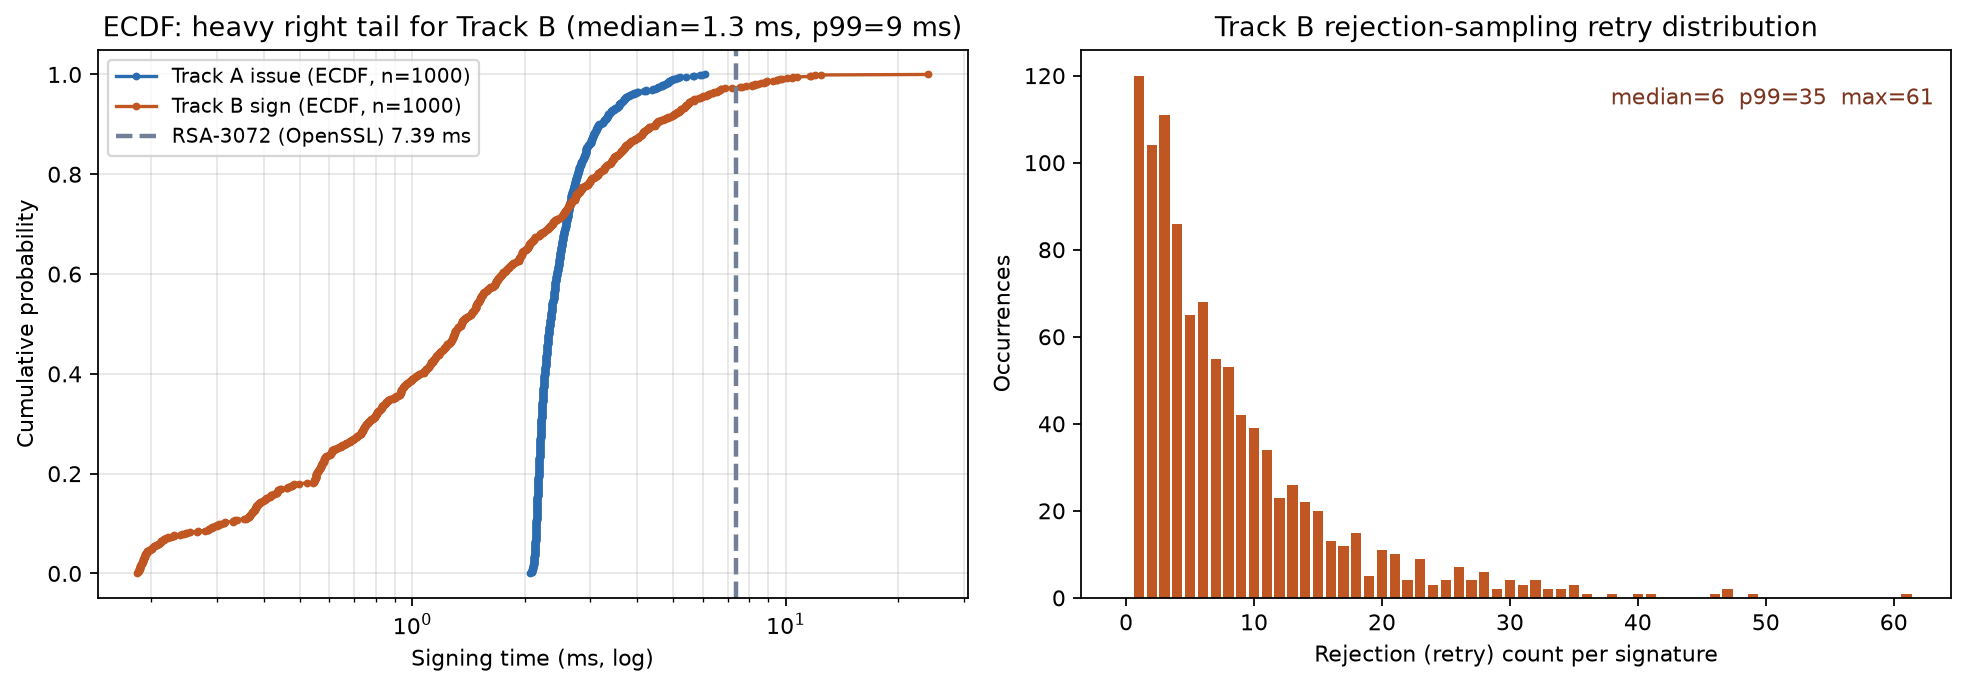
\includegraphics[width=\linewidth]{fig5_timing.png}
  \caption{E2.  Left: empirical CDF of signing time (log axis) for Track A
  issue and Track B sign (n=1000 each) with the constant RSA-3072 value for
  reference; the Track B heavy tail is visible (median 1.3~ms, p99 9~ms).
  Right: histogram of Track B rejection-retry counts
  (median 6, p99 35, max 61).}
  \label{fig:perf}
\end{figure}

\begin{figure}[t]
  \centering
  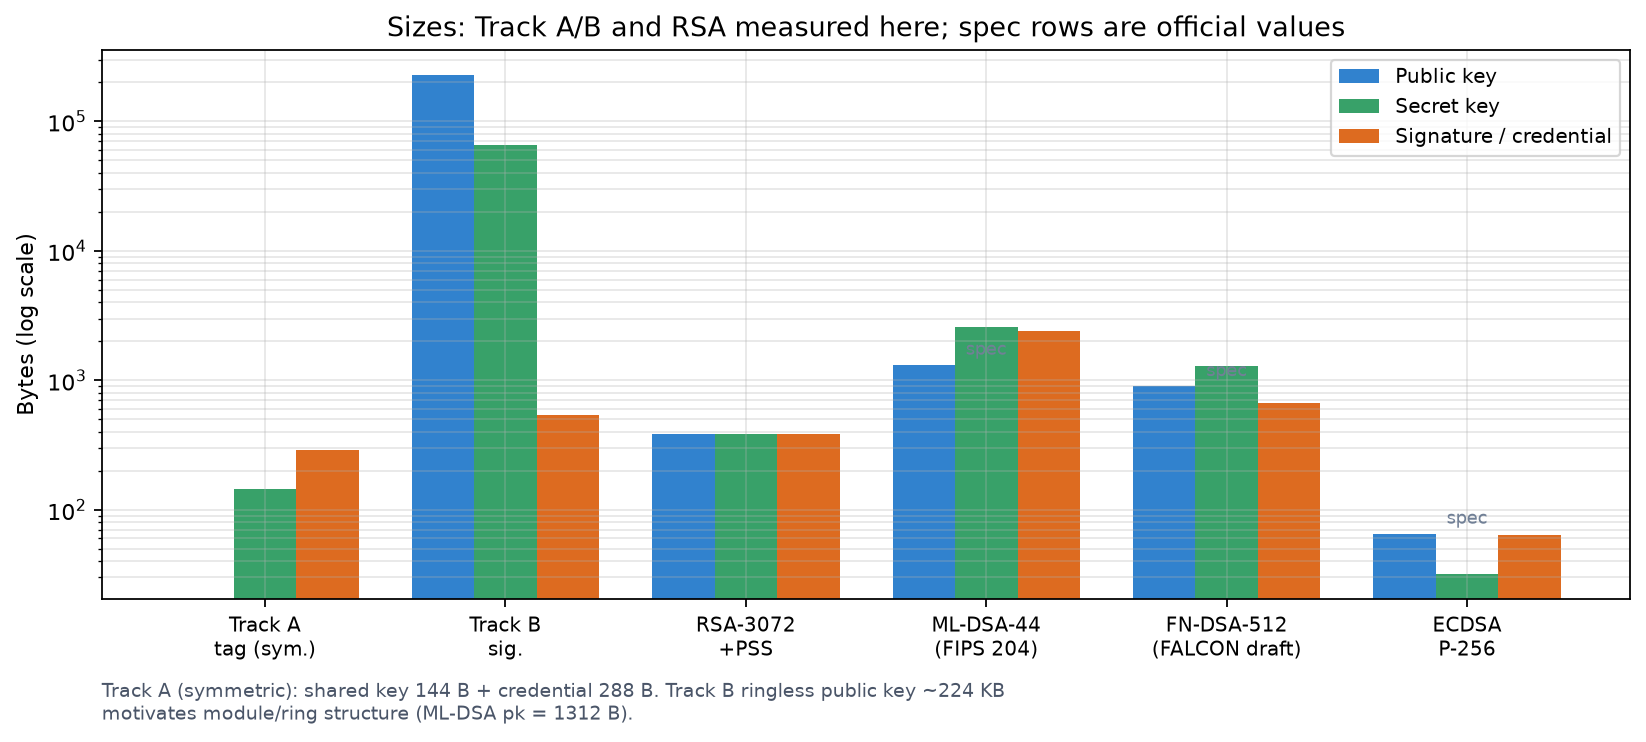
\includegraphics[width=\linewidth]{fig4_sizes.png}
  \caption{Public-key, secret-key, and signature/credential sizes (log axis).
  Track A/B and RSA rows are measured here; the NIST/FALCON rows are official
spec values (FN-DSA-512 from FALCON v1.2).
  The ringless Track B public key ($\approx 224$~KB) is the engineering
  motivation for module/ring-structured instantiations such as ML-DSA
  (pk 1312 B).}
  \label{fig:sizes}
\end{figure}

\subsection{E4: blockchain ledger scenario}
We simulate a single node receiving a block of $N=1000$ transactions of 64~B
payload each and verifying sequentially.  The ledger inflation factor is the
ratio of signature overhead to payload; verification TPS is derived from the
E2 median verify times.  Table~\ref{tab:block} reports the results.  Track A
adds $4.5\times$ and Track B $8.5\times$ overhead at measured verification
throughput of about $10\,000$ and $6\,300$ TPS respectively, both faster than
the measured RSA-3072-PSS signing-oriented baseline on this machine.  For the
NIST reference rows we use official signature sizes (FN-DSA-512:
FALCON v1.2 / FN-DSA draft values) and literature-order
verification costs (not measured here): ML-DSA-44 inflates by $37.8\times$,
FN-DSA-512 by $10.4\times$, and ECDSA P-256 is the $1.0\times$ baseline.  These
orders of magnitude reproduce the pattern reported by post-quantum migration
surveys~\cite{survey-pq-blockchain-2025,pq-transition-2026}: signature size,
not verification arithmetic, dominates ledger growth.

\begin{table}[t]
\centering
\caption{E4: per-transaction overhead and single-node verification throughput
for a block of 1000 transactions of 64 B each.  Rows marked (ref.) use official spec sizes (FN-DSA-512: FALCON v1.2 / FN-DSA
draft) and literature-order times, not measurements on this machine.}
\label{tab:block}
\begin{tabular}{lcc}
\toprule
Scheme & Inflation vs.\ payload & Verify TPS (median) \\
\midrule
Track A tag (measured)        & $4.5\times$  & $10\,235$ \\
Track B signature (measured)  & $8.5\times$  & $6\,262$ \\
RSA-3072-PSS (measured)       & $6.0\times$  & $7\,407$ \\
ML-DSA-44 (ref.)              & $37.8\times$ & $\sim 20\,000$ \\
FN-DSA-512 (ref.)             & $10.4\times$ & $\sim 12\,500$ \\
ECDSA P-256 (ref.)            & $1.0\times$  & $\sim 100\,000$ \\
\bottomrule
\end{tabular}
\end{table}

\begin{figure}[t]
  \centering
  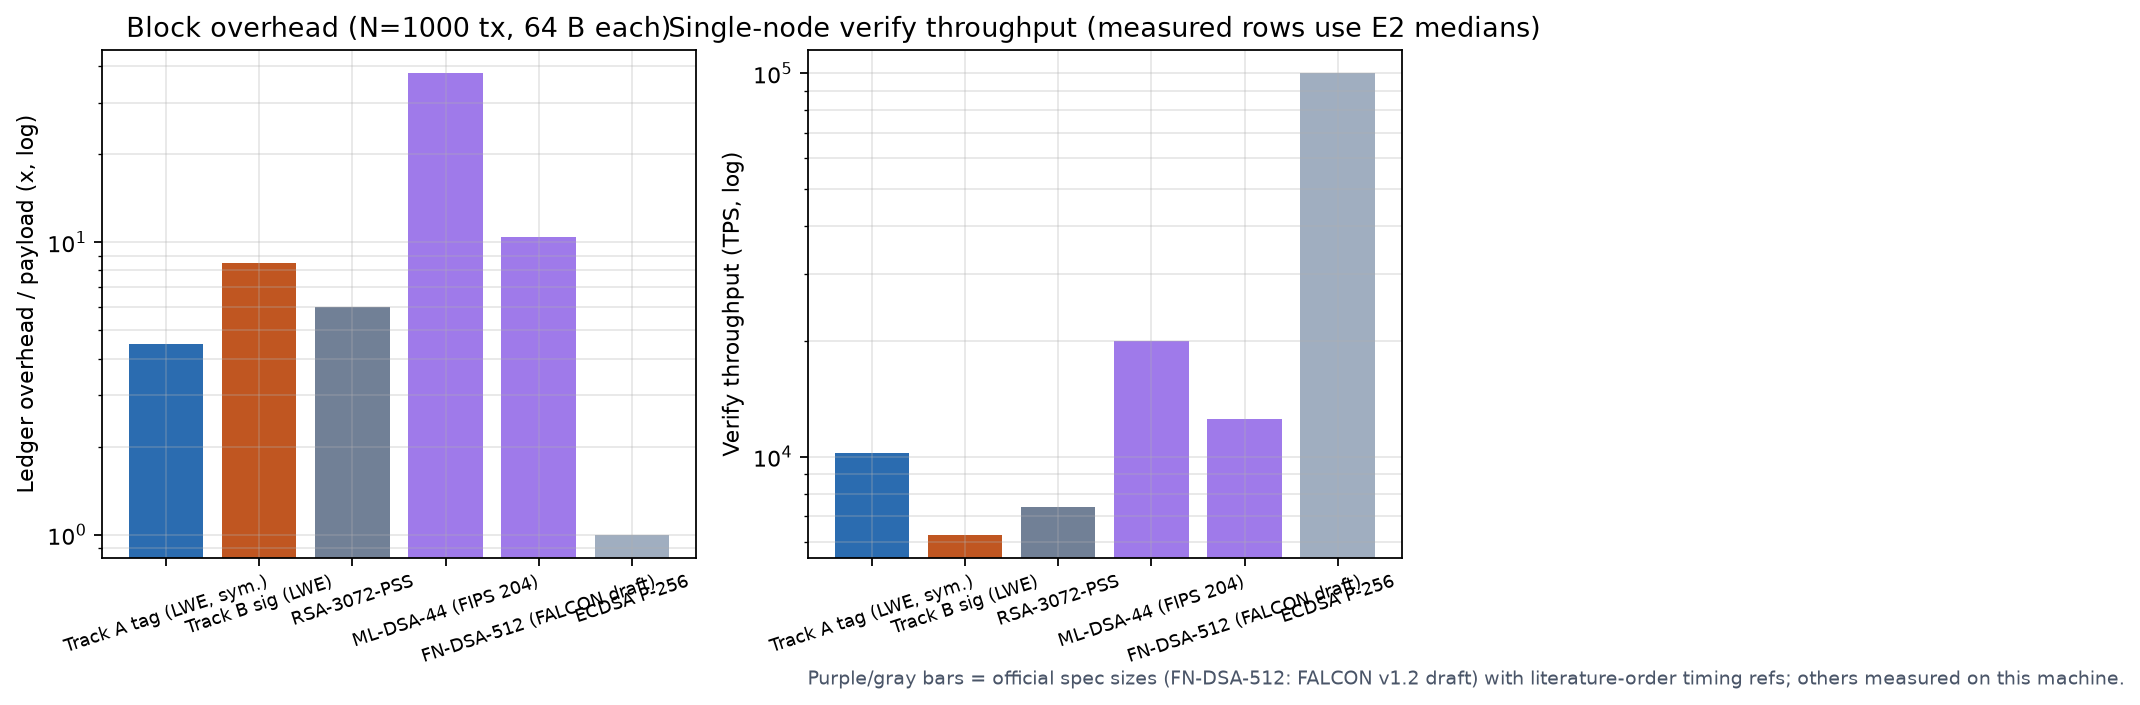
\includegraphics[width=\linewidth]{fig6_blockchain.png}
  \caption{E4.  Left: ledger-inflation multiple over the raw 64-B payload;
  right: single-node verification TPS (measured rows use E2 medians; purple/gray
  bars are official-size/literature-time references).}
  \label{fig:block}
\end{figure}

\section{Results Summary and Discussion}\label{sec:results}

The experiments support four high-level observations.

\begin{itemize}
\item \textbf{Correctness is clean at the tested scale.} Track A achieves
  $1.0000$ on all three correctness groups, and the threshold sweep shows a
  wide operating margin ($V=8$ sits above the empirical residual max of 6 and
  below any observed tamper residual).  Track B likewise achieves $1.0000$
  across 1000 valid, 1000 tampered, 1000 random-forgery, and 1000
  single-byte-mutation trials.
\item \textbf{Estimator and scaled attack agree qualitatively.} Recovery rates
  fall when dimension or noise grows and rise when more same-instance samples
  accumulate, matching the estimator's relative predictions.  The agreement is
  trend-level; per-point noise (see the 95\% CIs and non-monotonicities in
  Figure~\ref{fig:n}) is expected at 8--12 trials and should not be read as a
  precise ``hardness curve.''
\item \textbf{Rejection sampling dominates the latency story.} The Track B
  signing distribution is long-tailed (median 1.36~ms, max 24.1~ms, worst case
  61 retries), confirming the critique in~\cite{mldsa-bench-2026} that mean-only
  reporting is misleading for designs with aborts.  Any production deployment
  must budget for worst-case latency or bound retries via larger $\kappa$ /
  better sampling.
\item \textbf{Size, not arithmetic, is the blockchain bottleneck.} At 64-B
  payloads, signatures inflate blocks by $4.5$--$37.8\times$, and the measured
  verification throughput is in the thousands of TPS.  The ringless Track B
  public key of $\approx 224$~KB is the clearest sign that module/ring
  structure (as in ML-DSA) is required for real deployment.
\end{itemize}

\subsection{Limitations}
\begin{itemize}
\item \textbf{Teaching-level security estimates.} Our estimator is a
  root-Hermite/core-SVP model; in the regimes used here it often saturates at a
  dimensional upper bound and cannot distinguish fine effects of $\sigma$ (as
  seen in Figure~\ref{fig:m}, right).  The reference cross-check of
  Section~\ref{sec:crosscheck} shows that in this saturated regime the
  teaching numbers overstate hardness by one to three orders of magnitude in
  bit terms, and we therefore treat them as trend indicators only.  A complete
  production-level re-derivation (default dual family, bit-level Track~B
  instance) remains future work.
\item \textbf{Python + NumPy implementation.} All lattice code is in pure
  Python/NumPy on integer arrays; timings include interpreter overhead, and the
  LLL attack is a double-precision implementation valid only in small
  dimensions.  Cross-language conclusions should rely on the OpenSSL/industry
  baselines and on the relative, not absolute, comparisons.
\item \textbf{No formal proofs.} We present textbook-level correctness and
  zero-knowledge arguments; a rigorous ROM/QROM treatment, including the
  message-derived matrix caveat of I2, is future work.
\item \textbf{Small attack trials.} E3 uses 8--12 instances per point under a
  time budget; the phase-transition observations are qualitative.
\end{itemize}

\section{Conclusion and Future Work}\label{sec:concl}

We presented a reproducible design-space study of two lightweight lattice-based
constructions for blockchain transactions, together with a parameter
methodology that cross-validates a teaching-level estimator against scaled LLL
embedding attacks, a transaction-derived matrix variant with explicit security
caveats, and an open benchmark suite (E1--E4, plus a Track B correctness test) aligned with current
methodological best practices.  The results show that (i)~the two layers of
evidence agree in trend, (ii)~rejection sampling creates a long tail that
benchmarks must report as distributions, and (iii)~signature/key size is the
dominant blockchain cost driver, strongly motivating structured lattices.

Future work proceeds along four axes: (1)~formal ROM/QROM security proofs,
including a treatment of message-derived matrices; (2)~module-LWE/SIS
instantiations with NTT for compact keys and constant-time implementations;
(3)~a complete lattice-estimator re-derivation of production parameters,
including the default dual-attack family and a bit-level Track~B instance
that respects the length-bound constraint of Section~\ref{sec:crosscheck};
and
(4)~batch verification and threshold-signature extensions (e.g.,
Ringtail-style protocols) with the same measurement protocol.

\section*{Reproducibility}
\begin{itemize}
\item \textbf{Repository:}
  \url{https://github.com/linmcneil/quantum-resilient-signature} (public).
\item \textbf{One-command pipeline:} \texttt{python scripts/run\_v2\_all.py}
  reproduces E1 (Track A), E1b (Track B correctness), E3, E2, E4, and all figures.
\item \textbf{Seeds:} E1 = 12345 (per-instance derived seeds), E3 = 20260908,
  E2 = 20260908 with scheme instance seeds 11 (Track A) and 22 (Track B);
  machine metadata is embedded in each \texttt{data/eval\_v2\_*.json} (including \texttt{eval\_v2\_e1b.json}).
\item \textbf{Artifacts:} raw per-sample timing (\texttt{samples\_ms}),
  rejection-count histograms, threshold sweeps, and JSON result schemas are in
  \texttt{data/}; figures in \texttt{docs/figures\_v2/} (Chinese) and
  \texttt{docs/figures\_en/} (English).
\end{itemize}

\bibliographystyle{plain}
\bibliography{refs}

\end{document}





